\documentclass{article}
\usepackage[utf8]{inputenc}
\usepackage{graphicx}

\title{Driving Behavior}
\author{
Ernesto Adrián Álvarez Salazar  A00227490\\
Carlos Javier Leal Beltrán  A01741355\\
Carlos Moisés Chávez Jiménez  A01637322\\
Luis Armando Salazar López  A01114901\\
}
\date{Agosto 2022 - Septiembre 2022}

\usepackage{listings}
\usepackage{color}

\definecolor{dkgreen}{rgb}{0,0.6,0}
\definecolor{gray}{rgb}{0.5,0.5,0.5}
\definecolor{mauve}{rgb}{0.58,0,0.82}

\lstset{frame=tb,
  language=Python,
  aboveskip=3mm,
  belowskip=3mm,
  showstringspaces=false,
  columns=flexible,
  basicstyle={\small\ttfamily},
  numbers=none,
  numberstyle=\tiny\color{gray},
  keywordstyle=\color{blue},
  commentstyle=\color{dkgreen},
  stringstyle=\color{mauve},
  breaklines=true,
  breakatwhitespace=true,
  tabsize=3
}

\begin{document}

\maketitle

\section{Introducción}
Una conducta agresiva al manejar es el factor principal en los accidentes vehiculares en carretera. Así lo reporta la "AAA Foundation for Traffic Safety", ya que dentro de 106,727 choques fatales en un periodo reciente de 4 años, el 55.7 porciento de estos involucró a conductores que cometieron una o más acciones agresivas al manejar. Por lo anterior, buscamos ¿Cómo predecir conductas agresivas al manejar de manera rápida y lo más precisa posible?

La conducción agresiva incluye el exceso de velocidad, las pausas repentinas y los giros bruscos a la izquierda o a la derecha. Todos estos eventos se reflejan en los datos del acelerómetro y el giroscopio. Por lo tanto, sabiendo que hoy en día casi todo el mundo posee un smartphone que tiene una gran variedad de sensores, hemos obtenido diversos datos gracias a una aplicación de recopilación de datos en android basada en los sensores del acelerómetro y el giroscopio.


\section{Tratamiento Inicial de los Datos}

Para comenzar a trabajar con los datos, es necesario que pasen por un proceso de preparación que nos permita obtener la mejor parte de ellos. Este proceso se divide en tres etapas: Limpieza, Transformación y Visualización. A continuación desglosaremos las fases involucradas a este proceso:

    \subsection{Limpieza de los datos}

        La limpieza es la primera y una etapa fundamental del tratamiento de la información. Aquí se busca eliminar la mayor cantidad de imperfecciones que pudieramos llegar a encontrar. Cosas como valores faltantes, datos fuera de rango, dividir la información disponible en "entrenamiento" y "pruebas", eliminar columnas innecesarias para el análisis, etc.
        En el caso de nuestra base de datos, no hicimos ninguna limpieza (de momento). Encontramos muchos valores atípicos en las variables relacionadas con el movimiento de los conductores (giroscopio y acelerometro), pero no los eliminamos. Al ser demasiados, puede generar que se vaya mucha información que resulte valiosa para nuestro modelo. La parte importante fue que no encontramos valores faltantes, ni columnas innecesarias. \\

        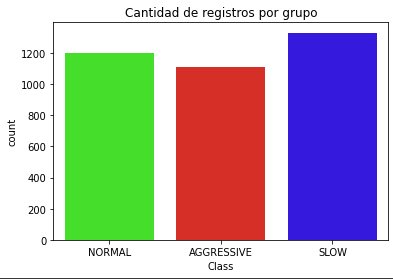
\includegraphics{images/Columnas.png} \\

        \textbf{Gráfico de barras sobre las clases disponibles en nuestro archivo de datos.} \\

    \subsection{Transformación de los datos}

        Una vez revisados los datos, entendemos que debemos transformarlos para generar gráficos y diagramas que faciliten la busqueda de patrones y la determinación de si será necesario un modelo predictor de regresión o de clasificación.
        Para esto, revisamos el dataframe con la información proporcionada. Encontramos que primero debemos ordenar los datos con base en el timestamp. Esta variable indica el tiempo con el que fueron realizadas las pruebas de los conductores. Se generaron dos observaciones por segundo, lo que indica que tenemos que separarlas para que queden enumeradas de uno en uno. Le restamos el primer valor del timestamp a todas las observaciones para dejar la inicial en 0, y separamos los valores para que quedaran enumeradas por el número de observación y no por el tiempo. Así no habría dos observaciones en el mismo segundo.
        En cuanto a lo demás, los datos venían en buenas condiciones, por lo que no tuvimos que arreglar valores núlos, ni valores que vinieran en formatos con los que no se puede trabajar.

    \subsection{Visualización de los datos}

       Esta etapa es un caso diferente. Pertenece igualmente a las fases previas al trabajo de los datos, pero no involucra descartar información. La visualización se encarga convertir los datos a diagramas o elementos gráficos que faciliten el entendimiento de la información. También para esta fase consideramos el cambiar algúnas variables de tipo de dato.

        Con base en los datos que contamos para relizar este trabajo, análizamos y decidimos qué diagramas utilizar para acercarnos al desarrollo de nuestro modelo. Seleccionamos los diagramas de correlación y cajas y bigotes. \\
        El diagrama de correlación nos permite conocer qué variables son más afínes a la variable que estamos intentado predecir. Lo cual nos ahorra mucho trabajo para seleccionar las variables que estarán involucradas en nuestro modelo. \\

        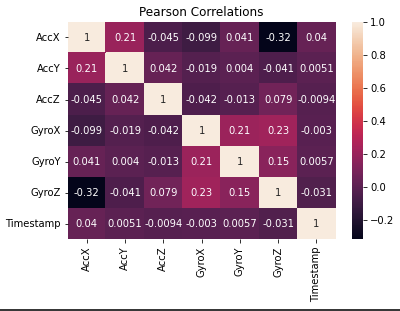
\includegraphics{images/Correlacion.png} \\

        \textbf{Gráfico de correlación entre nuestras variables.} \\
        
        El diagrama de cajas y bigotes nos permitió conocer si hay valores atípicos en nuestros datos con respecto a las variables independientes. De esta forma nosotros podemos descartar estos valores para hacer un modelo más ajustado y apegado a la realidad. Pero, para este caso particular, no debemos hacerlo. Al ser tantos este tipo de valores, el eliminarlos podría maquillar los datos y generar un modelo erroneo.\\

        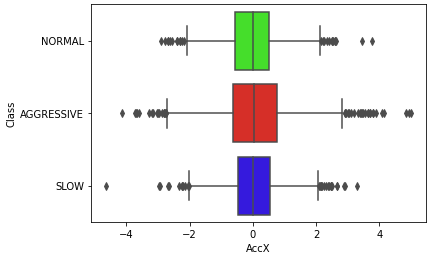
\includegraphics{images/Cajas y Bigotes AccX.png} \\

        \textbf{Gráfico de cajas y bigotes sobre la variable de aceleración "Acc X".} \\

\section{Desarrollo del modelo con los datos}

Habiendo trabajado ya con las primeras partes de los datos, ya podemos sacar conclusiones en cuanto a los patrones que buscamos, el cómo vamos a trabajar con los datos, cuántos datos requerimos para predecir y qué modelo elegir. A este punto, ya podemos definir la hipotesis que buscamos comprobar con nuestro modelo. \\

    \textbf{Hipotesis Nula: Se puede predecir el comportamiento y el peligro de un conductor con base en observaciones de tipos sobre su conducción: los cambios en la aceleración total (suma de las aceleraciones en las tres dimensiones) y los cambios en el giro total (suma del giro en las tres dimensiones).} \\
        
    \subsection{Busqueda de patrones}

        La visualización nos permitió entender que no estamos buscando un modelo nos prediga una clase con base a los parametros, sino un conjunto de observaciones que nos permita clasificar el tipo de conductor con base en la información de como conduce. 
        
        Al momento de análizar los gráficos que obtuvimos de los datos, encontramos algunos comportamientos y patrones que nos pueden acercar al desarrollo del modelo. Vimos que el comportamiento del conductor agresivo es cambiante constantemente y extremo en cuanto a los cambios de aceleración y direccion en todas las direcciones. Para comprobar esto, sacamos el valor total de las tres dimensiones de la aceleración y el giro para generar un grafico que nos permita comprobar nuestra hipotesis.

        \includegraphics{images/Aceleración Total.png} \\

        \textbf{Gráfico de Lineas sobre la suma de las aceleraciones en las tres dimensiones del acelerómetro.} \\

        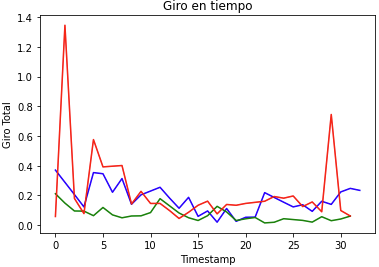
\includegraphics{images/Giro Total.png} \\

        \textbf{Gráfico de Lineas sobre la suma del giro en las tres dimensiones del giroscopio.} \\

        Como vimos en los anteriores gráficos, notamos que los valores del conductor agresivo se disparan y cambian constantemente. Esto simplemente nos muestra que nuestra hipotesis en cuanto a la inestabilidad y capacidad de predicción con base en los cambios de aceleración y el giro se comprueba. Lo anterior nos da una idea de lo que buscamos en nuestro modelo, y nos da una pauta de lo que podemos hacer para generar un modelo eficiente.

        Otra cosa que también nos ayudó a encontrar patrones, fue el sacar la raíz de las sumatorias de los cuadrados y las aceleraciones. De esta forma obtenemos un valor único para la aceleración y el giro de cada dirección. Los resultados que obtuvimos fueron los siguientes: \\

        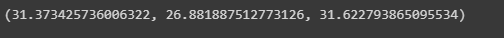
\includegraphics{images/Slow_Acc.png} \\

        \textbf{Aceleración total en cada dimensión para el conductor agresívo.} \\

        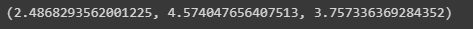
\includegraphics{images/Slow_Gir.png} \\

        \textbf{Giro total en cada dimensión para el conductor lento.} \\

        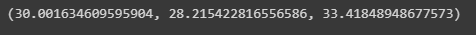
\includegraphics{images/Mid_Acc.png} \\

        \textbf{Aceleración total en cada dimensión para el conductor agresívo.} \\

        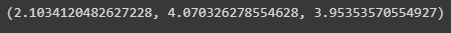
\includegraphics{images/Mid_Gir.png} \\

        \textbf{Giro total en cada dimensión para el conductor medio.} \\

        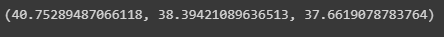
\includegraphics{images/Agg_Acc.png} \\

        \textbf{Aceleración total en cada dimensión para el conductor agresívo.} \\

        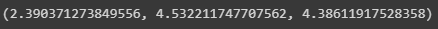
\includegraphics{images/Agg_Gir.png} \\

        \textbf{Giro total en cada dimensión para el conductor agresivo.} \\

        Analizándo los resultados, el giro no nos dijo mucho en cuanto a diferencias. Los datos son muy parecidos en cuanto a los tres tipos de conductores. Pero, podemos ver que sí hay una diferencia notable en la aceleración. Especificamente en las dimensiones Y y Z. Lo cual nos indica que podemos utilizar esas variables representativas para probar diferentes modelos y obtener el que tenga una mayor eficiencia.
        

    \subsection{Desarrollo del modelo}

        Para comenzar el desarrollo es necesario primero definir si sera de regresión o de clasificación. Este será de clasificación, nosotros esperamos recibir determinada cantidad de observaciones tomadas el manejo de un conductor, y determinar si qué tipo de conductor es. Teniendo definido lo anterior, es importante determinar cuántas observaciones serán necesarias para que el modelo haga la predicción. 
        
        Para calcular la cantidad de observaciones suficientes pensamos en que lo mejor es determinarlo con base en los datos que nos dan para test. Dividiendo la cantidad de datos entre las tres clases, ajustamos los datos para que nos den valores divisores similares. De esta forma encontramos el máximo común divisor de los datos y así determinamos la cantidad mínima de datos que necesitamos de un conductor para determinar si puede llegar a ser peligroso para los otros automovilistas.

        Teniendo definida la cantidad de datos mínima, podemos empezar a probar diferentes modelos para comparar la efectividad, y encontrar el más adecuado para esta situación. \\

        Teniendo los datos listos para trabajar, con los patrones descubiertos y la hipotesis definida; comenzaremos la busqueda del modelo con la mayor eficiencia. Dentro de los modelos que probaremos están \textbf{Random Forest} , \textbf{KNN} y \textbf{Decision Tree}.

        \subsubsection{Decision Tree}

            El primer candidato son los arboles de decisión. Este divide los datos entre todas sus caracteristicas para clasificar al valor que se ingresa en una categoria. 
            
            Siendo el caso de nuestros conductores, el modelo crea diferentes nodos de decision donde se va clasificando el dato hasta que encaje con las caracteristicas de un conductor. 

            Algunas ventajas de este candidato son que es muy facil de entender el funcionamiento, es válido tanto para variables cuantitativas y cualitativas y no requiere amplia preparación de los datos.

            Una de sus desventajas es que es inestable, un cambio en los datos desencadenaria en una reorganización del arbol.

            Con esto dicho, pasaremos a probar este modelo. Intentamos probarlo pasandole diferentes variables, desde una sola hasta todas las disponibles. El mejor resultado obtenido fue con todas las variables utilizadas: \\

            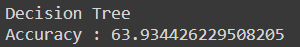
\includegraphics{images/Decision.png} \\

            \textbf{Resultado Arboles de Decision.} \\
            

        \subsubsection{KNN}

            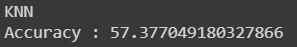
\includegraphics{images/KNN.png} \\
    
            \textbf{Resultados KNN.} \\

        \subsubsection{Random Forest}

            Por último está Random Forest. Este desarrolla múltiples árboles de decisión y los combina para obtener una predicción más precisa y estable. En general, mientras más árboles haya en el bosque, más robusto será.

            En este algoritmo se agrega algo aleatoriedad adicional al modelo, mientras crece los árboles, en lugar de solo buscar la característica más importante al dividir un nodo, busca la mejor característica entre un subconjunto aleatorio de características. Lo cual nos da como resultado una amplia diversidad que por lo general resulta en un mejor modelo. \\

            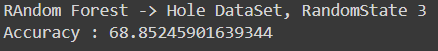
\includegraphics{images/RandomForest.png} \\
    
            \textbf{Resultados Random Forest.} \\

\section{Evaluación del modelo con los datos de prueba}

    Sample \\

    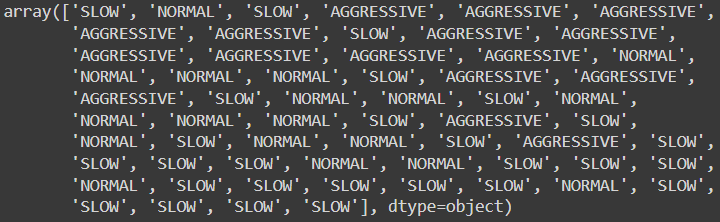
\includegraphics{images/ResultsDecision.png} \\
    
    \textbf{Resultados Arboles de Decision con datos de prueba.} \\

    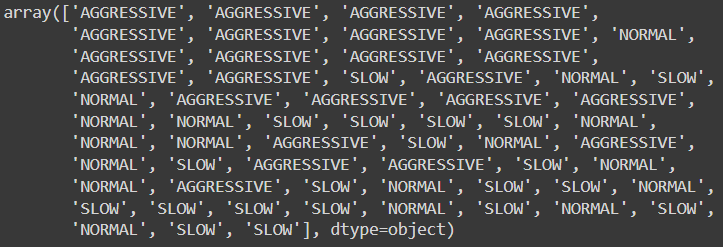
\includegraphics{images/ResultsKNN.png} \\
    
    \textbf{Resultados KNN con datos de prueba.} \\

    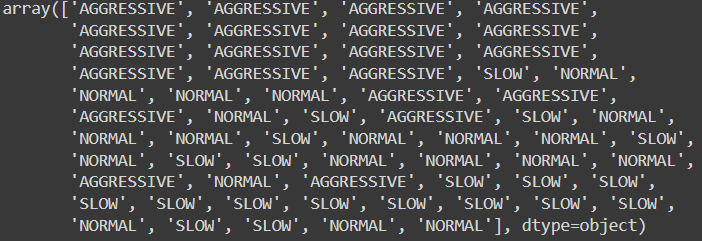
\includegraphics{images/ResultsRandom.png} \\
    
    \textbf{Resultados Random Forest con datos de prueba.} \\

\end{document}
